\chapter{Descrizione del Progetto}
\label{cap:descrizione}

\textit{\indent Questo capitolo fornisce il background tecnico essenziale per comprendere il progetto, analizza le problematiche delle tecnologie coinvolte e illustra l'idea fondamentale alla base del lavoro svolto.}

\section{Background}

~\\
\indent Questa sezione illustra il funzionamento e i principi fondamentali delle tecnologie chiave del progetto.
Quest'ultime costituiscono la base essenziale per la comprensione di questo studio. 

\subsection{Protocolli di Trasporto Tradizionali}
~\\
\indent Nel panorama dei \gls{protocolli di rete}\glsfirstoccur, i \gls{protocolli di trasporto}\glsfirstoccur \emph{TCP} (Transmission Control Protocol) e \emph{UDP} (User Datagram Protocol) hanno svolto e svolgono tutt'ora un ruolo fondamentale sin dalla nascita di Internet.
Questi protocolli sono stati la spina dorsale delle comunicazioni per decenni, supportando una vasta gamma di servizi e applicazioni.\\
In particolare \emph{TCP}, con la sua affidabilità e il suo controllo di flusso, ha svolto un ruolo fondamentale nelle comunicazioni che richiedevano l'integrità dei dati, mentre \emph{UDP} ha trovato il suo spazio nei servizi che privilegiavano la velocità rispetto all'affidabilità. 
Tuttavia, con l'evoluzione delle nuove tecnologie e la creazione di nuovi protocolli, le limitazioni di questi protocolli sono diventate sempre più evidenti. Nella concezione di base di \emph{TCP} e \emph{UDP}, ideata agli inizi del 1970, non erano state previste le sfide delle reti moderne, 
caratterizzate da:  
\begin{itemize}
    \item Connesioni mobili e variabili;
    
    \item Necessità di ridurre la latenza;
    
    \item Proliferazione di dispositivi IOT;
     
    \item Requisiti di sicurezza sempre più vincolanti.
\end{itemize}

\noindent Queste nuove sfide hanno evidenziato una serie di problematiche nei protocolli. La consapevolezza di questi limiti ha portato alla ricerca di nuove soluzioni, cercando di superare le inefficienze pur mantenendo tutti i punti di forza.
Questi studi hanno portato alla creazione di nuovi protocolli come \emph{QUIC}\glsfirstoccur ed a estensioni come \emph{MPTCP}\glsfirstoccur, che cercano di far fronte alle sfide del mondo moderno offrendo prestazioni migliori, maggiore sicurezza e flessibilità.
\\
\\
Nelle sezioni successive esamineremo in dettaglio alcune parti di \emph{TCP} e \emph{UDP}, per poi esplorare come \emph{QUIC} e \emph{MPTCP} si propongono di risolvere e superare le inefficienze presenti e le possibili ripercussioni.

\subsubsection{TCP (Transmission Control Protocol)}
~\\
% Fonte https://www.ietf.org/rfc/rfc793.txt %
\indent Il \emph{Transmission Control Protocol (TCP)}, come anticipato nella sezione precedente, è uno dei protocolli cardine su cui si basa la comunicazione su Internet. Dato il suo ruolo e la vasta gamma di funzioni che offre, un'analisi completa del suo funzionamento e della sua costituzione richiederebbe un'analisi approfondità che va oltre lo scopo di questa tesi. Pertanto, in questa sezione, ci concentreremo solo su alcuni aspetti specifici del TCP che sono fondamentali per la comprensione del nostro studio su \emph{QUIC}. 
In particolare, esamineremo nel dettaglio :
\begin{itemize}
    \item Caratteristiche principali di una connessione \emph{TCP};
    
    \item Il processo di \emph{Handshake} \glsfirstoccur;
    
    \item Il meccanismo di \emph{Ritrasmissione \glsfirstoccur};
    
    \item I metodi utilizzati per garantire la sicurezza dei dati.
\end{itemize}

\paragraph{ Caratteristiche principali}
\noindent Il \emph{Transmission Control Protocol} si distingue come un protocollo orientato alla connessione. Questa sua caratteristica significa che, prima di qualsiasi scambio di dati, deve essere stabilita una connessione dedicata tra il \emph{client \glsfirstoccur} e l'\emph{host\glsfirstoccur}.
Questa peculiarità è alla base di molte delle sue funzionalità avanzate, tra cui:
\begin{description}
    \item[Affidabilità] Viene utilizzato il meccanismo degli \emph{acknowledgements} \glsfirstoccur per garantire la corretta consegna dei segmenti;

    \item[Controllo di Errore] Implementa un sistema di verifica della integrità dei dati tramite il meccanismo degli \emph{checksum} \glsfirstoccur;
    
    \item[Controllo di Flusso e Congestione] Utilizza il sistema delle \emph{sliding window} \glsfirstoccur per ottimizzare il flusso di dati e diminuire il numero di segmenti ritrasmetti in caso di situazione di congestione.
\end{description}

\noindent Queste funzionalità si riflettono sulla struttura stessa di un segmento TCP, come si può vedere nella Figura \ref{fig}. Segue una breve descrizione di alcune delle sezioni a noi necessarie:

\begin{itemize}
\item \textit{\textbf{Source Port - Destination Port}}: Identificano rispettivamente il numero della porta di origine e destinazione .
\item \textit{\textbf{Sequence Number}}: Definisce il \emph{sequence number}, che indica la posizione del primo segmento TCP all'intenro del flusso. Inoltre se il \emph{control bits SYN \glsfirstoccur} è presente allora il \emph{sequence number} rappresenta il \emph{initial sequence number (ISN)} e il primo otteto successivo avrà come \emph{sequence number ISN+1};
\item \textit{\textbf{Acknowledgement Number}}: Se il \emph{control bits ACK \glsfirstoccur} è presente questo campo contiene il valore del prossimo \emph{sequence number} che il ricevente del segmento si aspetta di ricevere;
\item \textit{\textbf{Control Bits}}: Sono dei bit utilizzati per il controllo del protocollo. 
\begin{itemize}
    \item \textit{\textbf{URG}}: Se impostato a 1 indica la presenza di dati urgenti.
    \item \textit{\textbf{ACK}}: Se impostato a 1 indica che l'\emph{acknowledgmen  number} è valido;
    \item \textit{\textbf{PSH}}: Se impostato a 1 indica che i dati devono essere elaborati dai livelli superiori.
    \item \textit{\textbf{RST}}: Se impostato a 1 indica che la connesione non è più valida;
    \item \textit{\textbf{SYN}}: Se impostato a 1 indica che il mittente vuole stabilire una connesione TCP;
    \item \textit{\textbf{FIN}}: Se impostato a 1 indica che il mittente vuole terminare la connessione TCP.
\end{itemize}

\item \textit{\textbf{Checksum}}: Valore utilizzato per verificare la validità del segmento. Si ottiene facendo il complemento a uno della somma complementare a uno a 16 bit dell'\emph{header}, del \emph{payload} e altri di valori.
\item \textit{\textbf{Data}}: Rappresenta il vero e proprio \emph{payload} da trasmettere.
\end{itemize}

\begin{figure}[!h]
\centering
\includegraphics[width=0.8\columnwidth]{descrizione/tcp/segmento}
\caption{Segmento TCP}
\label{fig}
\end{figure}

\noindent È importante quindi notare che per costruzione il protocollo identifica univocamente una connesione TCP con una tupla composta da 4 elementi:

\begin{center}
    \small
    $[\text{Indirizzo IP sorgente}, \text{Porta sorgente}] \leftrightarrow [\text{Indirizzo IP destinazione}, \text{Porta destinazione}]$
\end{center}

\noindent Questa struttura offre diversi vantaggi. Permettere a un singolo \emph{host} di accettare più connessioni contemporaneamente da diversi \emph{client}, e viceversa. 
Inoltre garantisce l'unicità di ogni connessione all'interno della rete.
\\
Tuttavia, questa rigida definzione comporta delle limitazioni significative. In quanto una qualsiasi modifica ad un elemento della tupla (ad esempio, un cambiamento di porta o una migrazione dell'indirizzo IP) comporta la terminazione della connesione esistente. Questo diventa ancora più limitativo nel contesto delle comunicazioni moderne dove i casi di \emph{multihoming \glsfirstoccur} e cambi frequenti di indirizzo IP sono sempre più comuni.
\\
\\
Questa problematica, come vedremo nelle prossime sezioni, è alla base di soluzioni come \emph{MPTCP (Multipath TCP)} e viene affrontata in modo indiretto anche in \emph{QUIC (Quick Udp Internet Connection)}.

\paragraph{ Handshake }
% https://it.wikipedia.org/wiki/Round_Trip_Time

\noindent Come accennato in precedenza, uno dei punti cardine del \emph{TCP} è la necessità di stabilire una connessione prima di qualsiasi scambio di dati. Questo processo, noto come \emph{three-way handshake} (o più semplicemente "stretta di mano in tre passaggi"), richiede lo scambio di tre messaggi tra \emph{host} e \emph{client}. La Figura \ref{handshake} illustra questo processo.

\begin{figure}[!h]
    \centering
    \begin{minipage}{0.48\textwidth}
        \centering
        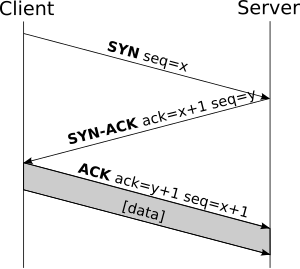
\includegraphics[width=0.75\columnwidth]{descrizione/tcp/three-way-handshake}
        \caption{\emph{three-way handshake}}
        \label{handshake}
    \end{minipage}
    \hfill
    \begin{minipage}{0.48\textwidth}
        \centering
        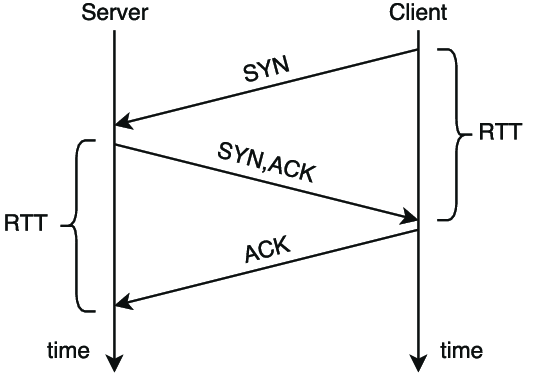
\includegraphics[width=0.90\columnwidth]{descrizione/tcp/rtt-handshake}
        \caption{\emph{RTT (Round Trip Time)}}
        \label{rtt}
    \end{minipage}
\end{figure}

\noindent Segue ora una breve spiegazione dei passaggi che avvengono in questo processo : 

\begin{enumerate}
    \item \textbf{Client invia un segmento SYN al Server}: Il segmento ha il campo \emph{SYN} impostato a 1 e il suo \emph{sequence number} contiene il \emph{ISN (Initial Sequence Number)} del Client;
    \item \textbf{Server invia un segmento SYN/ACK al Client}: Il Server risponde con un segmento i cui campi \emph{SYN} e \emph{ACK} sono impostati a 1. Il suo \emph{sequence number} contiene un nuovo valore y mentre l'\emph{Acknowledgement number} contiene il valore \emph{ISN+1};
    \item \textbf{Client invia un segmento ACK al Server}: Il Client risponde inviando un segmento il cui campo \emph{ACK} è impostato a 1 e l'\emph{acknowledgement number} è dato da \emph{y+1}.
\end{enumerate}

\noindent Tutti i segmenti utilizzati in questa fase hanno il campo \emph{data} vuoto, ossia sono solamente degli \emph{header}. 
Oltre a stabilire la connessione, l'\emph{handshake} riveste un ruolo fondamentale in vari aspetti della comunicazione TCP.
Non solo permette di sincronizzare i \emph{sequence number}, ma fornisce anche una base inziale per misurare il \emph{RTT (Round Trip Time)} \glsfirstoccur (Figura \ref{rtt}), che è essenziale per ottimizzare il controllo di flusso e la gestione della congestione della rete.

\paragraph{ Ritrasmissioni }

\noindent La gestione degli errori nel \emph{TCP} è un argomento estremamente complesso che necessiterebbe di uno studio dedicato. 
Tuttavia, ciò va oltre allo scopo di questa tesi e per motivi di spazio non verrà discusso. Pertanto ci limiteremo a descrivere brevemente il meccanismo di ritrasmissione, necessario per comprendere alcuni concetti della tesi.
\\\\
\noindent Il \emph{TCP} è un protocollo progettato per garantire l'affidabilità nella trasmissione dei dati. La ritrasmissione dei segmenti persi o danneggiati è uno dei meccanismi chiave per raggiungere questo obbiettivo. Questo processo si basa sulla logica degli \emph{acknowledgements}. Quando un segmento viene inviato, il mittente attende una conferma di ricezione (\emph{ACK}) dal destinatario. Se questa conferma non viene ricevuta entro un determinato intervallo di tempo, chiamato \emph{RTO (Retransmission TimeOut) \glsfirstoccur}, il mittente assume che il segmento sia stato perso e lo ritrasmette.
In particolare, è importante sapere che il calcolo del RTO è dinamico e dipende fortemente dal \emph{RTT} e da numerosi altri valori. 
\\\\
\noindent(Si puo' dedicare piu' spazio a questa sezione approndendo casistiche e meccanismi ulteriori)
\\\\
\noindent(Forse fuori tema e da rimuovere)(inerente nel caso si testasse sulle reti mobili)
\\
Sono numerose le cause che possono provocare la perdita di un pacchetto. Nel caso delle reti mobile ciò può accadere in punti diversi dell'infrasstruttura. Nel caso il segmento venga perso tra il client e la stazione base in \emph{RAN \glsfirstoccur} è compito del \emph{link layer} occuparsi della ritrasmissione. Questo significa che, se il pacchetto venisse perso un numero di volte ma poi venisse ricevuto, il TCP non rileverebbe alcun pacchetto perso ma solo un aumento del \emph{RTT}.
\paragraph{ Sicurezza }

\noindent Nella sua forma nativa, il protocollo \emph{TCP}, non offre meccanismi di sicurezza come autenticazione, integrità dei dati o confidenzialità. Infatti, \emph{TCP} non implementa alcuna funzionalità di crittografia o altri sistemi con lo scopo di proteggere i dati durante la trasmissione.
Per colmare questa mancanza, vengono utlizzati protocolli aggiuntivi come il \emph{Transport Layer Security (TLS)} e il \emph{Secure Sockets Layer (SSL)} (suo predecessore). Questi protocolli crittografici operano al \emph{livello di presentazione \glsfirstoccur} dello schema \emph{ISO/OSI \glsfirstoccur} e di conseguenza ad un livello superiore rispetto al \emph{TCP}.
Forniscono entrambi le funzionalità di sicurezza essenziali, garantendo una comunicazione protetta e affidabile.
\\\\
Nel contesto di questo studio, ci concentreremo in particolare sul protocollo \emph{TLS 1.3}, l'ultima versione di esso. Esamineremo brevemente la nuova procedura di handshake (Figura \ref{tlsHand}), essenziale per negoziare i parametri di sicurezza e stabilire una comunicazione cifrata.
\begin{figure}[!h]
    \centering
    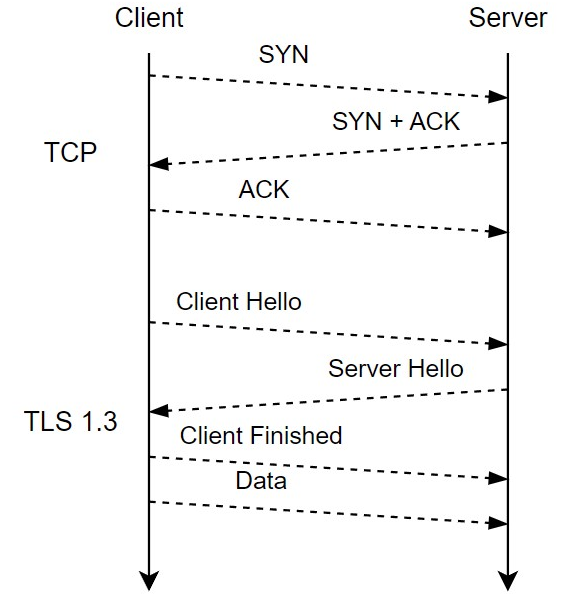
\includegraphics[width=0.7\columnwidth]{descrizione/tcp/tls-handshake}
    \caption{Nuovo Handshake (da modificare)}
    \label{tlsHand}
\end{figure}

\noindent Segue ora una breve spiegazione dei nuovi passaggi che avvengono in questo processo:
\begin{enumerate}
    \item \textbf{Client invia un messaggio ClientHello al Server}: Il messaggio contiene una lista dei cifrari supportati dal client;
    \item \textbf{Server risponde con un messaggio ServerHello al Client}: Il Server risponde con un messaggio che contiene: 
    \begin{itemize}
        \item  Il cifrario selezionato tra quelli inviati dal Client;
        \item  La chiave pubblica del server per l'algoritmo di scambio chiavi scelto.
    \end{itemize}
    Segue poi il messaggio \emph{Certificate}, che include il certificato del server, e un messaggio \emph{Finished} che conclude la sua parte dell'\emph{handshake};
    \item \textbf{Client invia un messaggio Finished}: Il Client dopo aver ricevuto il messaggio \emph{Finished} dal Server possiede tutte le informazioni necessarie per confermare il completamento dell'\emph{handshake} e invia a sua volta un messaggio \emph{Finished} per confermare il termine di tale operazione.
\end{enumerate}

\noindent È importante notare che con il \emph{TLS 1.3} si ha un \emph{2RTT}, ovvero vengono richiesti due \emph{Round Trip} prima dell'effettivo invio dei dati. 

\subsubsection{UDP (User Datagram Protocol)}
% https://datatracker.ietf.org/doc/html/rfc768
~\\
\indent Dopo aver esaminato brevemente il \emph{Transmission Control Protocol (TCP)},
procediamo ora all'analisi del \emph{User Datagram Protocol (UDP)}. 
Diversamente dal \emph{TCP}, questo protocollo si distingue per la sua semplicità e la minor complessità, offrendo un approccio più diretto alla trasmissione dei dati.
\\
Nonostante la sua relativa semplicità, una trattazione esaustiva dell'UDP andrebbe comunque oltre gli scopi di questa tesi. 
Di conseguenza ci concentreremo sulla struttura di un \emph{datagramma {UDP}} descritto in Figura \ref{udp-datagram}.
\\
\begin{figure}[!h]
    \centering
    \includegraphics[width=0.7\columnwidth]{descrizione/udp/segmento}
    \caption{Datagramma UDP (Da modificare)}
    \label{udp-datagram}
\end{figure}

\noindent Si può facilmente notare che l'\emph{header} di un datagramma \emph{UDP} è notevolmente più semplice rispetto a quello di un segmento \emph{TCP}.
In quanto questo è composto da soli quattro campi, i quali sono :  
\begin{itemize}
    \item \textit{\textbf{Source Port - Destination Port}}: Identificano rispettivamente il numero della porta di origine e destinazione. In questo caso il campo relativo alla \emph{source port} può essere omesso ed in tal caso settato a 0.
    \item \textit{\textbf{Lenght}}: Questo campo specifica la lunghezza in byte dell'\emph{header} e del \emph{payload}. La lunghezza minima è di 8 \emph{bytes} mentre il limite superiore è di 65,607 \emph{bytes}.
    \item \textit{\textbf{Checksum}}: Questo campo è opzionale e può essere usato per effettuare dei controli di errore sul datagramma.
\end{itemize}

Aggiungere che questo rispecchjia a pieno il suo campo di utilizzo in quanto un header senza overhead implica veloicita etc etc
\subsection{QUIC}

Qua c'è molto da dire

Da pensare ai capitoli 

\subsection{MPTCP}

Qua c'è molto da dire

Da pensare ai capitoli 

\section{I problemi e l'Idea}

I problemi di Quic e le nostre idee.


